\section{A Customized Programming Environment}
\label{sec:environment}

The features that influence the experience of the learning programmer are not limited to the programming language used. 
The \emph{tools} used to write, analyse and evaluate the code have a paramount relevance for this experience, and therefore for the success of the programming courses.

We decided to embed the Wollok language in an integrated programming environment, whose features are designed having in mind the specific needs of novice programmers.
The visual appearance and graphic structure of the Wollok IDE are similar to those of several Eclipse distributions. 
In turn, the set of tools it provides is, mostly, the result of a selection from the broader collection standard to mainstream industrial IDEs like Eclipse, Visual Studio or the Idea series, and a subsequent adaptation of some features to enhance their value to early course attendants.
In this way, we aim to make both the programming experience more appealing to the students, and the transition to later courses and work environments softer; while giving adequate support to the learning process through the same tools.

\medskip
In addition, we decided to include two tools which are not bundled in standard industrial IDE distributions. 
One of these is the REPL that we already described in Section~\ref{sec:wollokLanguage}.
The other is the automatic generation of \emph{static diagrams}, cfr. Fig.~\ref{fig:outline}, that are higlhy customizable in terms of which elements (classes/objects, methods, attributes) include, and also their spatial distribution.

\begin{figure}[ht]
 \centering
 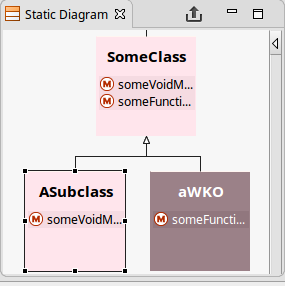
\includegraphics[scale=0.5]{../images/staticDiagram.png}
 \caption{\small Static diagram.}
 \label{fig:outline}
\end{figure}

We mention some standard features bundled in the IDE:
\begin{itemize}
\item 
A powerful \textbf{code editor}, with syntax highlighting, proper indentation, and automatic insertion of closing delimiters. The editor offers also smart \emph{content assist} in several situations, e.g. \texttt{super} and \texttt{self} sends and messages to be sent to a WKO.
%The the extent in which options can be elucidated given the absence of explicit type information in the Wollok 

\item
Automatic \textbf{detection of errors and warnings} integrated into the IDE, focused on situations that novice programing tend to experience. Some examples: unused or never-assigned variables, instantiation of abstract classes, absence of matching methods for messages sent to WKOs, \texttt{super} and \texttt{self} sends. In some cases, automatic fixes are suggested.

\item
Visual \textbf{test runner} for the tests that are part of Wollok syntax, described in Section~\ref{sec:wollokLanguage}.
\end{itemize}
